\documentclass[a4paper]{scrreprt}

\usepackage[german]{babel}
\usepackage[utf8]{inputenc}
\usepackage[T1]{fontenc}
\usepackage{ae}
\usepackage{amssymb}
\usepackage{graphicx}
\usepackage{hyperref}

\begin{document}

m\title{BS Zusammenfassung}
\author{Benedict Hauck, Fedor Scholz}
\maketitle

\tableofcontents
\vspace{1cm}

\chapter{01aIntro}

\section{Was ist ein Betriebssystem?}

\begin{itemize}
	\item Vermittler zwischen Benutzer und Computer
	\item Ziele
		\begin{itemize}
			\item Benutzerprogramme ausfuehren und dem Benutzer das Loesen von Problemen erleichtern
			\item Computer benutzbarer machen
			\item Hardware des Computer effizient nutzen
		\end{itemize}
	\item Vier Komponenten eines Computersystems
		\begin{itemize}
			\item Benutzer
			\item System- und Anwendungsprogramme
			\item Betriebssystem
			\item Hardware
		\end{itemize}
	\item Betriebssysteme verteilen Ressourcen
		\begin{itemize}
			\item Verwaltung aller Ressourcen
			\item Entscheidung bei konfligierenden Anfragen fuer effizientes und faires Benutzen der Ressourcen
		\end{itemize}
	\item Betriebssysteme kontrollieren
		\begin{itemize}
			\item Kontrolle von Ausfuehrungen von Programmen um Fehler und ungeeignetes Benutzen des Computers zu verhindern
		\end{itemize}
	\item Das Programm, welches immer laeuft, ist der Kernel. Alles andere ist entweder ein System- oder Anwendungsprogramm
	\item Das bootstrap program wird beim Starten oder Neustarten geladen
		\begin{itemize}
			\item Wird in ROM, EPROM oder FLASH als firmware gespeichert
			\item Initialisiert alle Aspekte des Systems, insbesondere die HW-Komponenten
			\item Laedt den Kernel und startet die Ausfuehrung
		\end{itemize}
\end{itemize}

\section{Organisation}

\begin{itemize}
	\item Ein oder mehr CPUs, device controllers verbinden sich ueber den Bus um Zugriff auf shared memory zu bekommen
	\item I/O-Geraete und CPU koennen gleichzeitig ausfuehren
	\item Jeder device controller ist zustaendig fuer einen Geraetetypen
	\item Jeder device controller hat einen lokalen Puffer
	\item CPU bewegt Daten vom/zum Hauptspeicher zu/von lokalen Puffern
	\item I/O ist vom Geraet zum lokalen Puffer des controllers
	\item device controller informiert CPU per interrupts, wenn er fertig ist
\end{itemize}


\section{Interrupts}

\subsection{Haeufige Funktionen von Interrupts}

\begin{itemize}
	\item interrupt gibt Kontrolle an interrupt service routine ueber einen interrupt vector, welcher die Adressen von allen service routines beinhaltet
	\item interrupt architecture muss Adresse der unterbrochenen Intruktion speichern
	\item Einkommende interrupts sind aus, wenn gerade ein anderer bearbeitet wird um lost interrupts zu verhindern
	\item trap ist ein interrupt, welcher von Software verursacht wurde (wegen eines Fehler oder durch eine Benutzeranfrage)
	\item Betriebssysteme sind interrupt driven
\end{itemize}

\subsection{Timer interrupts}

\begin{itemize}
	\item Time interrupts um endlose Schleifen und Prozesse zu verhindern
	\item Wird nach bestimmter Zeitspanne ausgefuehrt
	\item Wird vor dem schedulen des Programm aufgesetzt
	\item Eingebettete Systeme haben Watchdog, welche bis 0 zaehlt und dann resettet
\end{itemize}

\subsection{Interrupt Handling}

\begin{itemize}
	\item Betriebssystem merkt sich Status der CPU, indem es Register und Programmzaehler speichert
	\item Legt Typ des interrupts fest
		\begin{itemize}
			\item polling
			\item vectored interrupt system
		\end{itemize}
\end{itemize}

\section{I/O Struktur}

\subsection{Synchrone oder blockende I/O}

\begin{itemize}
	\item Nachdem I/O beginnt, geht die Kontrolle erst nach Fertigstellung der I/O wieder zum Benutzerprogramm
	\item Wait instruction laesst die CPU idlen
	\item Meistens nur ein I/O Request gleichzeitig
	\item Polling
	\item Signal
	\item Callback function
\end{itemize}

\subsection{Direct Memory Access Structure}

\begin{itemize}
	\item Fuer high-speed I/O, damit diese mit fast der Geschwindigkeit des Hauptspeichers Informationen uebertragen koennen
	\item Device Controller uebertraegt Daten in Bloecken vom Puffer direkt in den Hauptspeicher ohne CPU Eingriff
	\item Nur ein interrupt pro Block
\end{itemize}

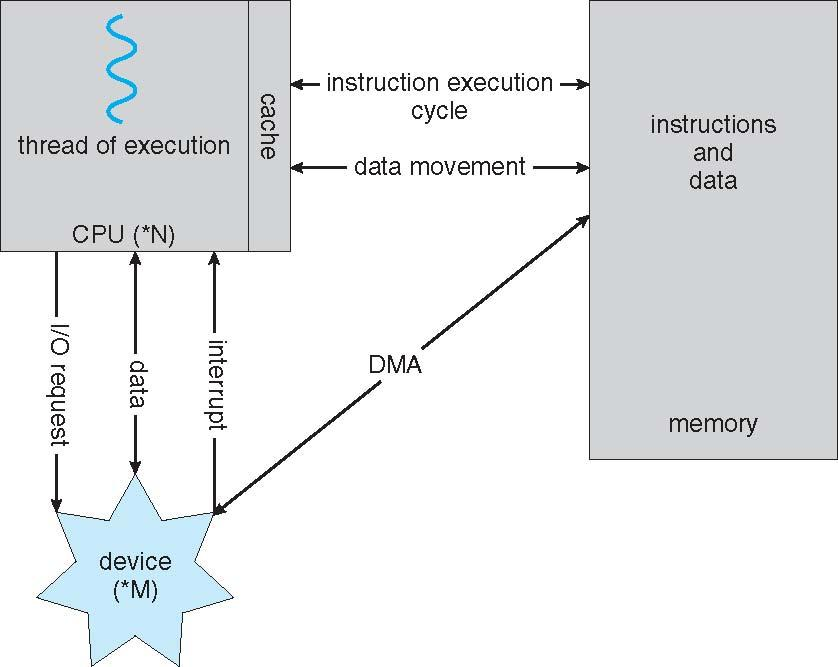
\includegraphics[scale=0.4]{dma.png}









\chapter{01bCProgramming}
\chapter{02OS}

\section{Monolithisches System}
Vorteile:
	\begin{itemize} 
		\item Einfacher Zugriff auf alle Systemdaten 
		\item Kosten von Modulinteraktionen sind niedrig
		\item Erweiterbar über Schnittstellen
		\item Vorhersehbares Verhalten 
	\end{itemize}
Nachteile:
	\begin{itemize}
		\item Kein Schutz zwischen System und Anwendung
		\item Instabil
	\end{itemize}

Beispiele:
	\begin{itemize}
		\item uCLinux, RTOSe, eCos
	\end{itemize}
	
\section{Mehrschichtiger Ansatz}
	\begin{itemize}
		\item Betriebssystem ist in n Schichten aufgeteilt
		\item Jede Schicht kann nur auf die Funktionen und Dienste von niedrigeren Schichten zugreifen 
			\begin{itemize} 
				\item Schicht 0 ist die Hardware
				\item Schicht n ist das Benutzerinterface
			\end{itemize}
		\item Einfachere Migration zwischen Plattformen
		\item Einfachere Evolution der Hardwareplattform
		\item Niedrigere Schichten implementieren Mechanismen
		\item Höhere Schichten implementieren meistens Policies
	\end{itemize}

\begin{center}
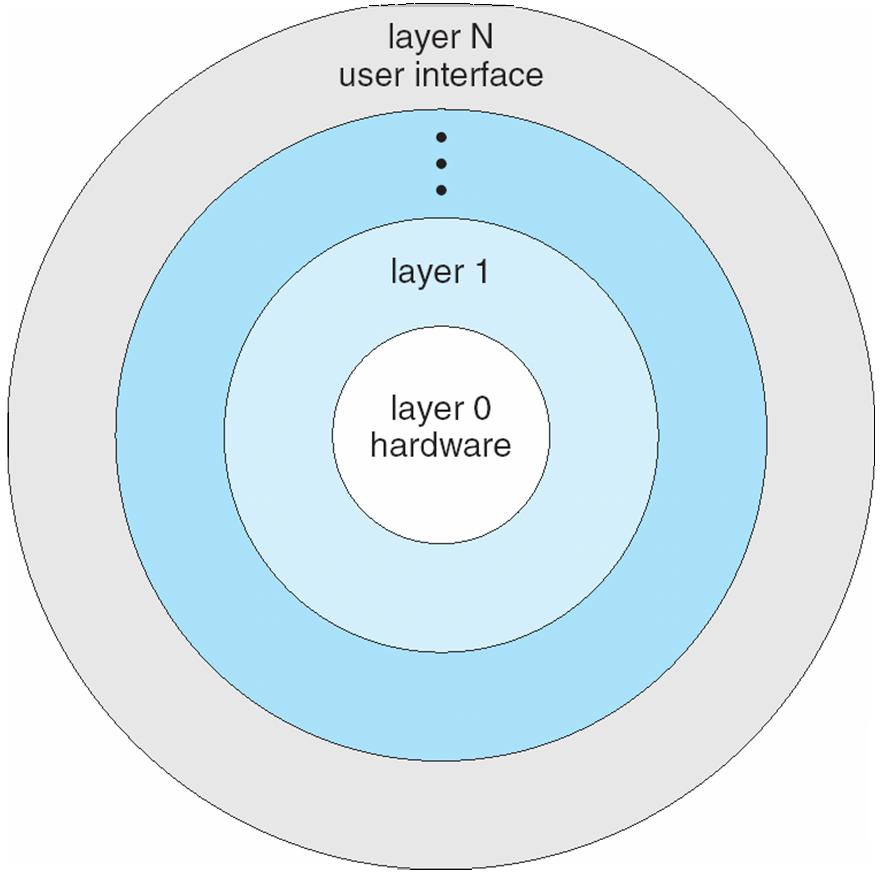
\includegraphics[scale=0.15] {schichtenmodell.png} 
\end{center}

Vorteile:
	\begin{itemize}
		\item Jede Schicht kann unabhängig getestet und verfiziert werden
		\item Korrektheit von Schicht n hängt nur von Schicht n-1 ab (einfacheres Debugging, einfachere Wartung)
	\end{itemize}

Nachteile:
	\begin{itemize}
		\item Nur unidirektionaler Schutz
		\item Beiseitige Abhängigkeit von Schichten verhindert strikte Schichtenbildung
	\end{itemize}
Beispiele:
	\begin{itemize}
		\item THE (Dijkstra), Multics(GE), VOCOS(EWSD)
	\end{itemize}
	
\section{Monolitische Kernels}
	\begin{center}
		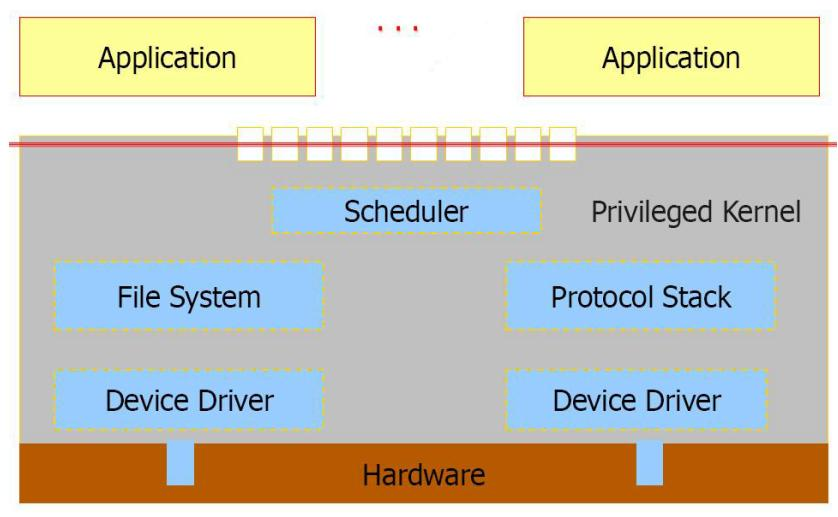
\includegraphics[scale=0.3] {monolithickernel.png}
	\end{center}
	Vorteile:
		\begin{itemize}
			\item "Gute" Performance
			\item Ausreichender Schutz zwischen Anwendungen
			\item Erweiterbar über Schnittstellen und statische/ladbare Module
		\end{itemize}
	Nachteile:
		\begin{itemize}
			\item Kein Schutz zwischen Kernel-Komponenten
			\item Nebeneffekte durch undokumentierte Interfaces
			\item Hohe Komplexität durch hohe gegenseitige Abhängigkeit
		\end{itemize}
	Beispiele
		\begin{itemize}
			\item Linux, Solaris
		\end{itemize}

\section{Microkernel Systeme}
	\begin{center}
		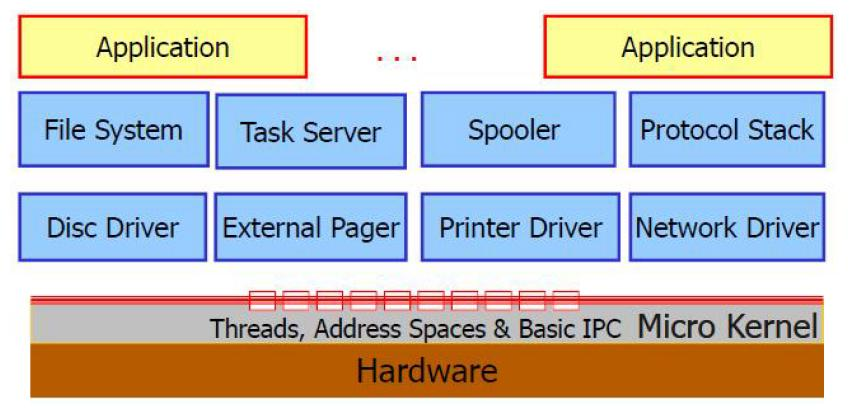
\includegraphics[scale=0.3] {microkernel.png}
	\end{center}

	\begin{itemize}
		\item Möglichst viel des Kernels in den "Benutzer" space packen
		\item Kommunikation erfolgt zwischen Benutzermodulen mit Nachrichtenweitergabe
	\end{itemize}
	
	Vorteile:
		\begin{itemize}
			\item Einfacher einen Microkernel zu erweitern
			\item Einfacher das Betriebssystem auf neue Architekturen zu portieren
			\item Zuverlässiger (es läuft weniger Code im Kernel-Modul
			\item Mehrere APIs vorhanden
			\item Verbesserte Robustheit und Sicherheit
			\item Einfacher zum Testen und Beweisen
			\item Verbesserte Wartbarkeit
		\end{itemize}
	Nachteile:
		\begin{itemize}
			\item Performance Unkosten durch Kommunikation von Benutzerspace zum Kernelspace 
			\item Zusätzliche Zersetzung
			\item Schlechte Erfahrungen mit IBMs Workplace OS (1991-1995)
		\end{itemize}

\section{Virtuelle Maschinen}
	\begin{itemize}
		\item Eine virtuelle Maschine nimmt den mehrschichtigen Ansatz und behandelt Hardware sowie den Kernel des Betriebssystems so als wären sie Hardware
		\item Eine virtuelle Maschine stellt ein identisches Interface zu der blanken, darunterliegenden Hardware
		\item Der Betriebssystem-Host kreiert die Illusion das ein Prozess sein eigenen Prozessor und (virtuellen Speicher) hat.
		\item Jeder Gast bekommt eine Kopie des darunterliegenden Computers zur Verfügung gestellt.
	\end{itemize}
	Vorteile:
		\begin{itemize}
			\item Mehrere Betriebssysteme können sich die gleiche Hardware teilen
			\item Gegenseitiger Schutz
			\item Nützlich für Development und Testen
		\end{itemize}
	\begin{center}
		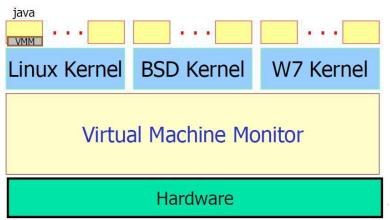
\includegraphics[scale=0.5] {virtualmachine.png}
		\\
		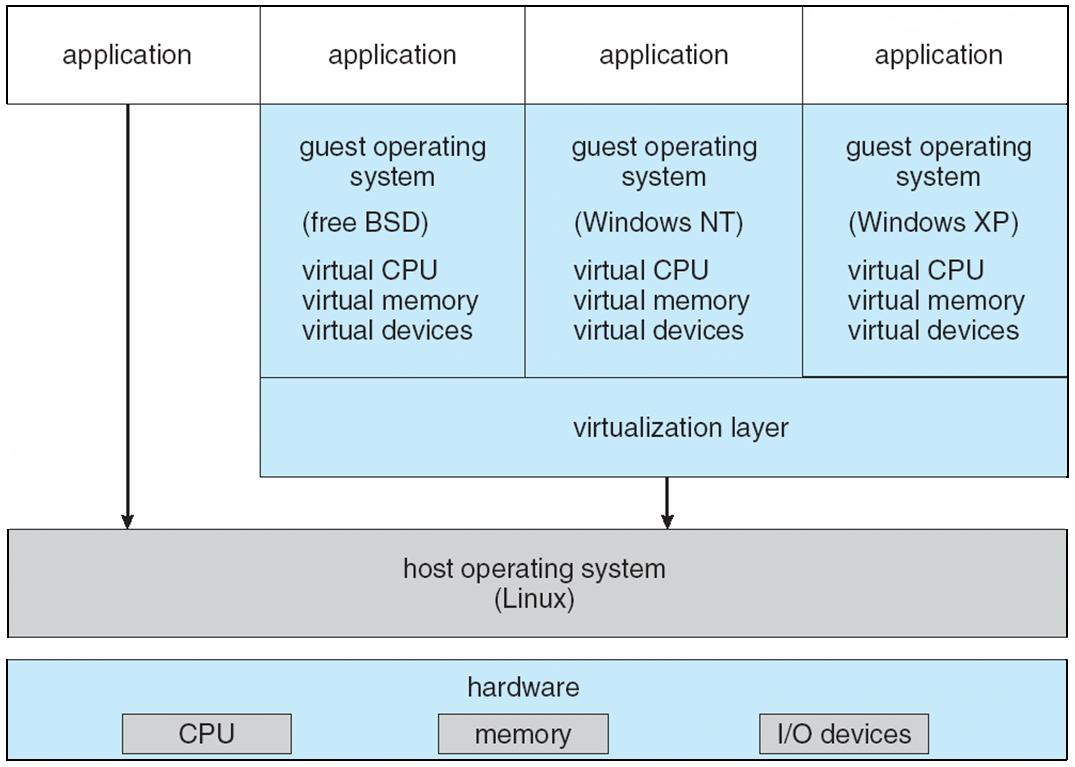
\includegraphics[scale=0.35] {vmwarearchi.png}
		\\
		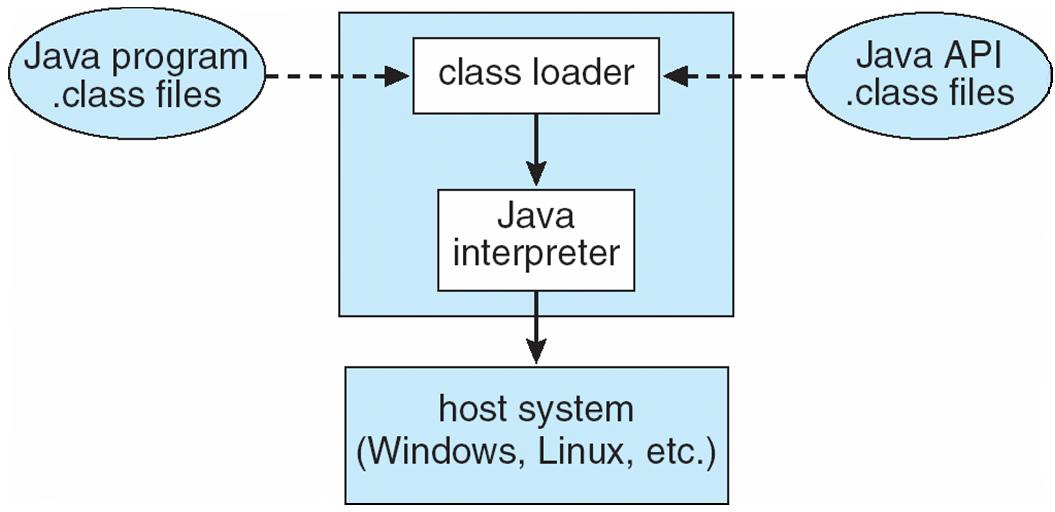
\includegraphics[scale=0.3] {javavm.png}
	\end{center}


\chapter{03aProcess-management}
\chapter{03bProcess-management-scheduling}
\chapter{04Process-coordination}
\chapter{05aMemoryManagement}
\section{Background}
\begin{itemize}
\item Damit ein Programm laufen kann muss es von der Platte in den Speicher gebracht und innerhalb des Prozesses plaziert werden.

\item Auf Hauptspeicher und Register kann nur die CPU direkt zugreifen.

\item Ein Register Zugriff beträgt einen CPU Takt (oder weniger)

\item Hauptspeicher kann einige Zyklen dauern.

\item Cache liegt zwischen Hauptspeicher und CPU Registern

\item Sicherheit des Speichers werden zur Sicherstellung korrek ausgeführter Operationen benötigt.

\end{itemize}

\subsection{Speicherpartitionierung}

Hauptspeicher wird normalerweise in zwei Partitionen unterteilt :
\begin{description}
\item[Resident operating system]\ \\ werden normalerweise im "`low memory"' mit  \textit{interrupt vector} gespeichert
\item[User processes]\ \\werden im "`high memory"' gespeichert
\end{description}

Register dienten dem Schutz der Benutzerprozesse untereinander und vor Veränderungen von Betriebssystemcode und Daten.
\begin{itemize}
\item "`Base register"' beinhalten den Wert der kleinsten physichen Adresse.
\item "`Limit register"' beinhalten den Umfang der logischen Adressen.
\end{itemize}

\begin{center}
		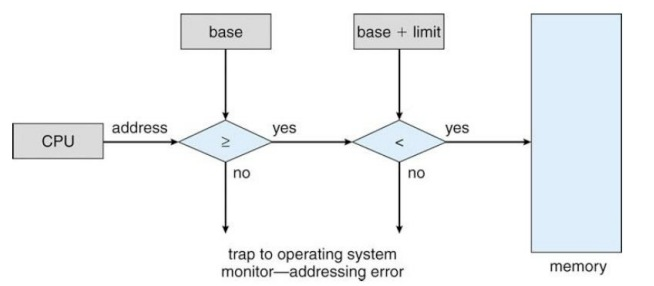
\includegraphics[scale=0.5] {baseandlimit.png}
\end{center}

\subsection{Einfacher Schutz mit \textit{base} und \textit{limit register}}

Ein Paar aus base und limit Registern definieren einen logischen Adressraum

\begin{center}
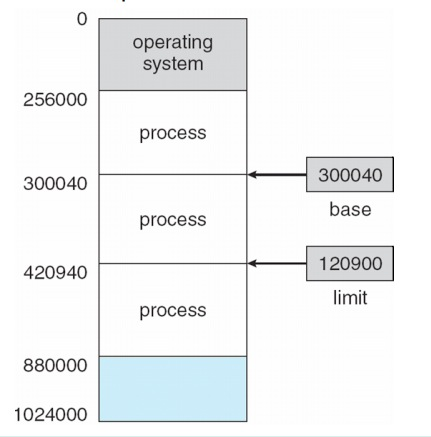
\includegraphics[scale=0.5]{baseandlimitprotection.png}
\end{center}


\section{Swapping}
\begin{itemize}
\item Ein Prozess kann temporär aus dem Speicher in einen Zusatzspeicher gewechselt werden und dann wieder zurück um die Ausführung fortzusetzen
\item \textbf{Zusatzspeicher (\textit{Backing store})} \ \\ Schneller Speicher, welcher groß genug ist um alle \textit{memory images} aller Nutzer unterzubringen. Er muss jedoch direkten Zugriff zu jenen bieten.
\item \textbf{Roll out, roll in} \ \\ Eine Swapping Variation für prioritätsbasierte scheduling Algorithmen: Prozesse niedriger Priorität werden mit Prozessen hoher Priorität ausgewechselt um somit geladen und ausgeführt werden können.
\item Hauptbestandteil der \textit{swap time} ist die \textit{transfer time}: Die totale Transferzeit ist direkt proportional zur Menge des ausgewechelten Speichers
\item Modifizierte Versionen von ˆ\textit{swapping} wird auf vielen System gefunden (z.B UNIX, Linux und Windows)
\item Das System führt eine \textit{ready queue} mit "`ready to run"'-Prozessen welche ein memory image im Speicher haben.

\end{itemize}

\begin{figure}[ht]
\centering
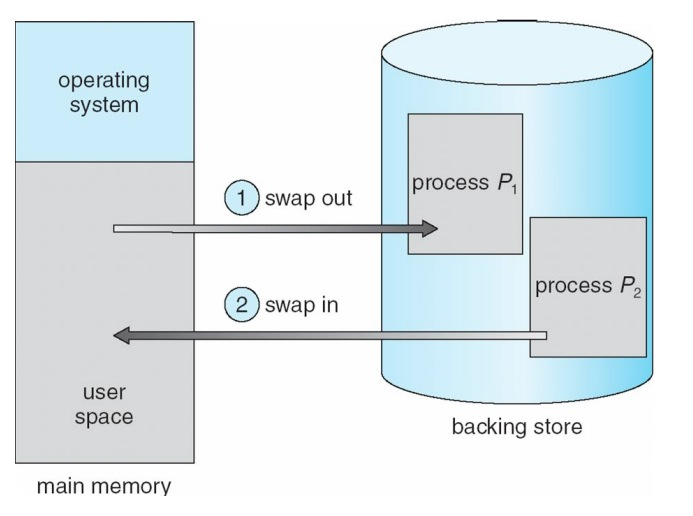
\includegraphics[scale=0.6]{swapping.png}
\caption{Schematik von Swapping}
\end{figure}

\section{Allocation}
\subsection{Zusammenhängende Allokierung (\textit{contiguous allocation)}}
\subsubsection{Multiple Partitions Allokierung}
\begin{itemize}
\item \textit{Hole}: Blöcke an verfügbarem Speicher. Löcher verschiedener Größe sind über den ganzen Speicher verteilt
\item Bei Ankunft eines Prozesses, wird Speicher von einem Loch, welches groß genug ist um den Prozess aufzufassen, allokiert
\end{itemize} Das Betriebssystem kümmert sich um Informationen über:

\begin{itemize}
\item[a)] allokierte Partitionen
\item[b)] freie Partitionen (Löcher)
\end{itemize}

\begin{figure}[ht]
\centering
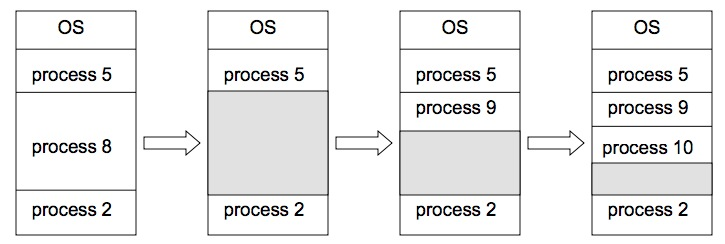
\includegraphics[scale=0.6]{allocation.png}
\caption{Schematik Speicherallokierung}
\end{figure}

\subsection{Dynamisches Speicher-Allokations Problem}
\textbf{Problem:} Wie befreidigt man Anfragen der Größe n von einer Liste mit freien Löchern?
\begin{itemize}
\item \textit{First-fit}: Allokiert das erste Loch, welches groß genug ist: schnellste Allokierungsstrategie, hinterlässt jedoch Löcher unterschiedlicher Größe
\item \textit{Best-fit}: Allokiert das kleinste passende Loch. Es muss jedoch die komplette Liste durchsucht werden, außer sie ist nach Größe sortiert. Hinterlässt die kleinsten Löcher.
\item \textit{Worst-fit}: Allokiert das größte Loch. Es muss die gesammte Liste durchsucht werden, hinterlässt die größten Löcher
\item \textit{Next-fit}: Nächst passendes Loch nach der letzten Allokierung
\item \textit{Buddy System}:
\begin{itemize}
\item Die Löcher werden in k Listen so einsortiert, dass die i-te Liste jeweils Löcher der Länge gleich $2^i/$ für i = 1,...,k enthält
\item Dabei können zwei benachbarte Löcher der i-ten Liste effizient zu einem  Loch der i+1-ten Liste zusammengefügt werden
\item Umgekehrt kann ein Loch der i-ten Liste einfach in zwei Löcher der i-1-ten Listen aufgeteilt werden
\item Löcher im Buddy-System können effizient mittels eines Binärbaumes dargestellt werden
\item Laufzeitverhalten: Zuweisen und Freigabe Block schneller als first/best-fit. Fragmentierungsbehandlung ist aufwändiger. Deshalb Lazy-\textbf{Buddy:Zusammenfügen "`selten"'}
\item Standard für Unix/Linux
\end{itemize}
\end{itemize}

\begin{figure}[ht]
\centering
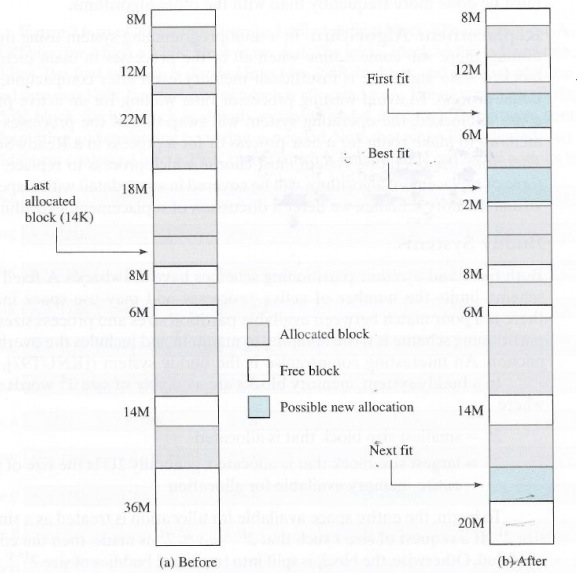
\includegraphics[scale=0.55]{allocationexample.png}
\caption{Beispiel vor und nach Allokierung eines 16Mbyte Blocks}
\end{figure}

\begin{figure}[ht]
\centering
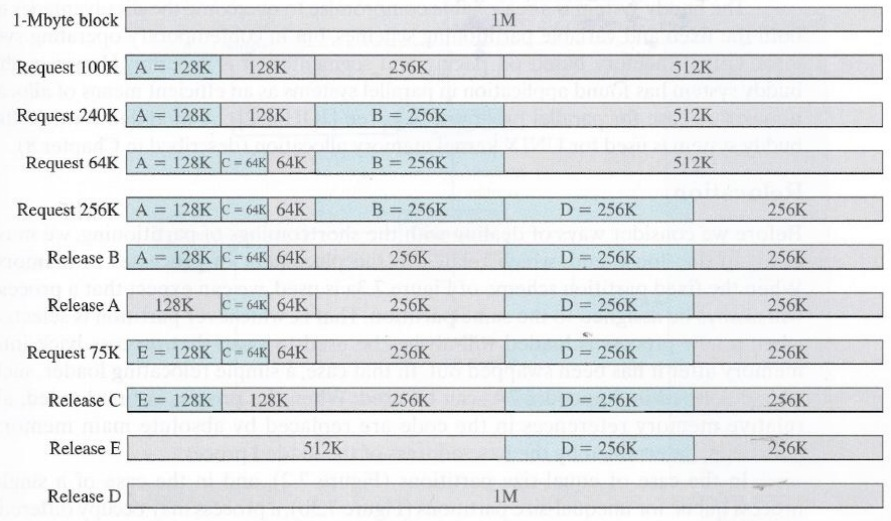
\includegraphics[scale=0.50]{buddysystem.png}
\caption{Beispiel Buddysystem}
\end{figure}
  \ \\
\begin{figure}[ht]
\centering
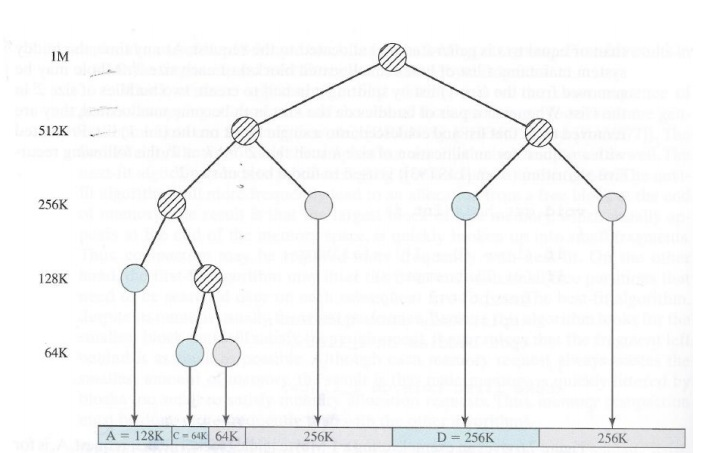
\includegraphics[scale=0.5]{buddysystemtree.png}
\caption{Darstellung Buddysystem als Baum}
\end{figure}
\newpage

\section{Relocation}
\subsection{Fragmentierung}
\begin{itemize}
\item \textbf{Externe Fragmentierung} - Es ist genügend Speicher vorhanden um eine Anfrage zu befriedigen, jedoch nicht zusammenhängend.
\item \textbf{Interne Fragmentierung} - Allokierter Speicher kann ein wenige größer als der angeforderte Speicher sein: Der Größenunterschied ist Speicherintern innerhalb einer Partition, wird jedoch nicht verwendet
\item Reduzierung externer Fragmentierung durch Verdichtung (\textit{compatction}):
\begin{itemize}
\item Vermische den Speicherinhalt um alle freien Speicher in einem großen Block zu sammeln
\item \textit{Compaction} ist nur dann möglich wenn die \textit{relocation} dynamisch und während der Durchführungszeit statt findet

\end{itemize}
\end{itemize}
\subsection{Addressbinding und "`Data to Memory"'}

\begin{itemize}
\item \textbf{Compile time}: Wenn der Speicherstelle  a priori bekannt ist, kann ein absoluter Code generiert werden. Muss jedoch recompiliert werden wenn der Startpunkt verändert wir.
\item \textbf{Load time}: Muss versetzbaren (engl.: \textit{relocatable}) Code generieren wenn die Speicherstelle zur Übersetzungszeit nicht bekannt ist.
\item \textbf{Execution time}: \begin{LARGE}
\textbf{lol wut kein plan, 5a, Folie 17}
\end{LARGE}
\end{itemize}

\subsection{Logische vs. Physicher Adressraum}

\begin{itemize}
\item \textbf{logische Adresse} - CPU generiert, auch als virtuelle Adresse bezeichnet
\item \textbf{physische Adresse} - von der Speichereinheit gesehene Adresse.

Logische und physische Adressen sind im Sinne von Kompilierzeit und "`load-time adress-binding-schemes"' gleich. Unterschied liegt in der "`execution-time adress-binding scheme"'
\end{itemize}

\subsection{Memory-Management Unit (MMU)}
\begin{itemize}
\item Hardware Geräte welche virtuellen auf physikalischen Adressen abbilden
\item Auf jede Adresse, die von einem Nutzerprozess generiert wurde, wird der Wert der relocation register addiert um die Hardwareadresse zu ermitteln.
\item Das Endnutzerprogramm setzt sich mit den logischen Adressen auseinander, nie mit den real physischen.
\end{itemize}


\section{Segmentation}
\section{Paging}
\chapter{05bMemoryManagement}
\chapter{05cMemoryManagement}
\chapter{06aFileSystems}
\chapter{06bFileSystems}
\chapter{07aImplementingFileSystems}
\chapter{07bImplementingFileSystems}
\chapter{08SecondaryStorageStructure}
\chapter{09IoSystems}

\end{document}
